\section{1. The Nature of  Classical Mechanics}
\begin{enumerate}
\item Discrete state machines: simplest example of dynamical system (directed graph)
\item To be valid in classical mechanics, dynamical law must be:
  \begin{enumerate}
  \item Deterministic (There's only one next state)
  \item Reversible (Conservation of information: there's only one previous state)
  \end{enumerate}
\item Even in a cycle, there's still one in-edge and one out-edge
\item There can be separate cycles: these correspond to conservation laws (The system stays in the cycle it started in.)
\end{enumerate}

\section{2. Motion}

\section{3. Dynamics}
$F = ma$
\section{4.    Systems of  More Than One Particle}
\begin{enumerate}
\item The force vector acting on a particle is determined by the locations of all the particles:
  \begin{align*}
    m_i\ddot{\x}_i = \vec{F_i} = \vec{F_i}(\x_1, \x_2, \ldots, \x_N).
  \end{align*}
\item Note that
  \begin{enumerate}
  \item There are $N$ such equations.
  \item Each equation is really 3 equations: one for each spatial dimension.
  \end{enumerate}
\item So, the {\it configuration space} is d$3N$-dimensional. Given a point in configuration space, we can compute the acceleration
  vector of each particle in the system.
\item But that is not enough to specify the evolution of the system: we need to know the current velocities (momenta)
  also.
\item So our {\it state space} is $6N$-dimensional \footnote{In physics, this full state space is called ``phase space'': ``configuration space plus momentum space
    equals phase space''.}.
\item Note that the dynamical law can be written
  \begin{align*}
    \vec{\dot{p}}_i = \vec{F_i} = \vec{F_i}(\x_1, \x_2, \ldots, \x_N).
  \end{align*}
\item A consequence of Newton's 3rd Law is that the net force on a closed system of  $N$ particles is zero.
\item Therefore the rate of change of momentum is zero: the law of \emph{conservation of momentum}.
\item Recall from chapter 1 the notion that cycles in a dynamical system correspond to conservation laws. Here we have
  an example:
  \begin{enumerate}
  \item We can label points in $6N$-dimensional state space according to the total momentum of the system.
  \item Conservation of momentum means that these partitions of state space are cycles / unconnected components of the
    graph.
  \end{enumerate}
\item So the system corresponds to a point $(\x, \vec{p})$ in a $6N$-dimensional state space. Our system evolves according
  to a trajectory $(\x(t), \vec{p}(t))$ in this state space. This trajectory never jumps between points
  with different values of total system momentum.

\end{enumerate}

\todo{Explain why the second-order DE is equivalent to two first-order
  DEs, i.e. why the $3N$ N2L equations are really $6N$ equations.}

\section{5. Energy}
\begin{enumerate}
\item Configuration $\x$ is a point in a $3N$-dimensional space.
\item Potential energy function $V(\x)$.
\item Force as negative derivative of PE $V(\x)$.
\item Time-derivative of PE + KE is zero under N2L.
\end{enumerate}
\section{6. The Principle of Least Action}

\subsection*{Definition of Action and Lagrangian}
The \textit{action} of a trajectory $x(t)$ for a single particle is
\begin{align*}
    \mathcal{A}[x]
    &=  \int_{t_0}^{t_1} \(\frac{1}{2}m\dot{x}(t)^2 - V\(x(t)\)\) \dt \\
    &= \int_{t_0}^{t_1} \(T - V\) \dt \\
    &= \int_{t_0}^{t_1} \Lag\(x(t), \dot{x}(t)\) \dt.
  \end{align*}

  \red{Why does he seem to deny that you need to know velocity for the Lagrangian? p 108, 109}

  \subsection*{The Principle of Least Action}
  The {\it principle of least action} states that the trajectory $x(t)$ that is taken is that for which the
  action is minimal (actually, a stationary point).

  \subsection*{N particles}
  For $N$ particles we have $N$ trajectory functions $x_1, \ldots, x_N$, and the action is a functional depending
  on all of them:

  \begin{align*}
    \mathcal{A}[x_1, \ldots, x_N]
    &=  \int_{t_0}^{t_1} \(\frac{1}{2}\sum_im_i\dot{x_i}(t)^2 - V(x_1(t), \ldots, x_n(t)\) \dt \\
    &= \int_{t_0}^{t_1} \(T - V\) \dt \\
    &= \int_{t_0}^{t_1} \Lag(x_1(t), \ldots, x_2(t), \dot{x_1}(t), \ldots, \dot{x_2}(t)) \dt.
  \end{align*}


  \subsection*{The Euler-Lagrange equations}
  The least action set of trajectories (trajectory of the system through configuration space) satisfies the
  following {\it at every point $t$ in time}.  :
  \begin{align*}
    \begin{cases}
      \ddt \pdLdxdOne - \pdLdxOne = 0 \\
      \vdots \\
      \ddt \pdLdxdN - \pdLdxN = 0
    \end{cases}
  \end{align*}
  \subsection*{Informal derivation of Euler-Lagrange equations}

  \subsubsection*{One-dimensional system}

  Consider a particle moving along a line. The (unknown) trajectory it follows is written as $x(t)$.

  The ``action'' for the system is the functional
  \begin{align*}
      \mathcal{A}[x]
      &= \int_{t_a}^{t_b} \Lag\( x(t), \dot{x}(t) \) \dt.
  \end{align*}
  \begin{theorem*}[Euler-Lagrange equations]
    The trajectory $x(t)$ that minimize $\mathcal{A}$ satisfies the following for all $t \in (t_a, t_b)$:
    \begin{align*}
      \ddt \pdLdxd = \pdLdx.
    \end{align*}
  \end{theorem*}
  \begin{proof} (sketch)

    We pretend that time is discrete and that the system evolves via $n$ instantaneous ``jumps'' each
    $\Delta t$ seconds apart, so that the particle visits locations $x_1, x_2, \ldots, x_n$ at clock
    ticks $1, 2, \ldots, n$.

    The discretized version of the functional we wish to minimize is
    \begin{align*}
      \mathcal{A}[\x]
      &= \sum_i \Lag\( x_i, \dot{x}_i \) \Delta t.
    \end{align*}
    Now, instead of seeeking a minimizing function in an infinite-dimensional function space, we are working in a
    finite-dimensional space: we need to find the values $x_1, \ldots, x_n$ that minimize the action. So we
    differentiate with respect to each $x_i$, set these derivatives equal to zero, and solve the resulting system
    of equations.

    In our discrete-time model, we make the following replacements: at the $i$-th clock tick, the position
    is $\frac{x_{i+1} + x_i}{2}$, and velocity is $\frac{x_{i+1} - x_{i}} {\Delta t}$, so we have
    \begin{align*}
      \mathcal{A}[\x]
      &= \sum_i \Lag\( \frac{x_{i+1} + x_i}{2}, \frac{x_{i+1} - x_i} {\Delta t} \) \Delta t.
    \end{align*}
    The partial derivative with respect to a particular $x_i$ involves only the $(i-1)$-th and $i$-th terms of the sum:
  \begin{align*}
    \frac{1}{\Delta t}\frac{\partial \mathcal{A}}{\partial x_i}
    &= \frac{\partial}{\partial x_i} \(
    \Lag\( \frac{x_i + x_{i-1}}{2}, \frac{x_i - x_{i-1}}{\Delta t} \) +
    \Lag\( \frac{x_{i+1} + x_i}{2}, \frac{x_{i+1} - x_{i}}{\Delta t} \) \) \\
    &=
    \frac{1}{2}\pdLdx\Big|_{x=x_{i-1}} + \frac{1}{\Delta t}\pdLdxd\Big|_{x=x_{i-1}} +
    \frac{1}{2}\pdLdx\Big|_{x=x_i}     - \frac{1}{\Delta t}\pdLdxd\Big|_{x=x_i} \\
    &= \(\frac{\pdLdx\Big|_{x=x_i} + \pdLdx\Big|_{x=x_{i-1}}}{2} \) -
      \(\frac{\pdLdxd\Big|_{x=x_i} - \pdLdxd\Big|_{x=x_{i-1}}}{\Delta t} \).
  \end{align*}
  In the limit $\Delta t \to 0$, (we claim that) the condition $\frac{\partial A}{\partial x_i} = 0$ for $i=1,\ldots, n$ becomes
  \begin{align*}
    0 = \pdLdx - \ddt \pdLdxd,
  \end{align*}
  for all $t$.
\end{proof}

\subsection*{Equivalence of Lagrange equations and Newton's second law}
\begin{exercise}
  Let $\Lag(x, \xdot) = \frac{1}{2}m\xdot^2 - V(x)$. Show that the Euler-Lagrange
  equation $\pdLdx = \ddt \pdLdxd$ is equivalent to Newton's law of motion $F = ma$.
\end{exercise}
\begin{proof}
  On the LHS we have $\pdLdx = -V'(x) = F$.

  We have $\pdLdxd = m\xdot$, therefore on the RHS we have $\ddt \pdLdxd = m\xddot = ma$.
\end{proof}


\subsection*{Generalized coordinates}
With ``generalized coordinates'' $q$ in place of $x$, this captures ``all of classical physics in a nutshell!
If you know what the $q_i$s are, and if you know the Lagrangian, then you have it all.''

\subsection*{Changing coordinate system}

In observer A's frame of reference, a particle is at $x$.

Observer B is moving relative to observer A according to a function $f(t)$.

In observer B's frame of reference, the particle is at $X = x - f(t)$.

According to observer $A$, the Lagrangian is $\frac{1}{2}m\xdot^2 - V(x)$, which under E-L leads to the
equation of motion $m\xddot = -V'(x)$ or $F = ma$.

According to observer $B$, the Lagrangian is $\frac{1}{2}m\(\dot{X}(t) + \dot{f}(t)\)^2 - V(X)$, which under
E-L leads to the equation of motion $m\(\ddot{X} + \ddot{f}\) = -V'(x)$, or $F = ma + m\ddot{f}$. So
observer $B$ sees a fictitious force $m\ddot{f}$, associated with their movement.

\subsection*{Change of coordinates Example 2}

Observer A (reference frame A) uses coordinates $x$ and $y$.

Observer B (reference frame B) uses coordinates $X$ and $Y$.

Reference frame B is rotating relative to A:

\begin{mdframed}
  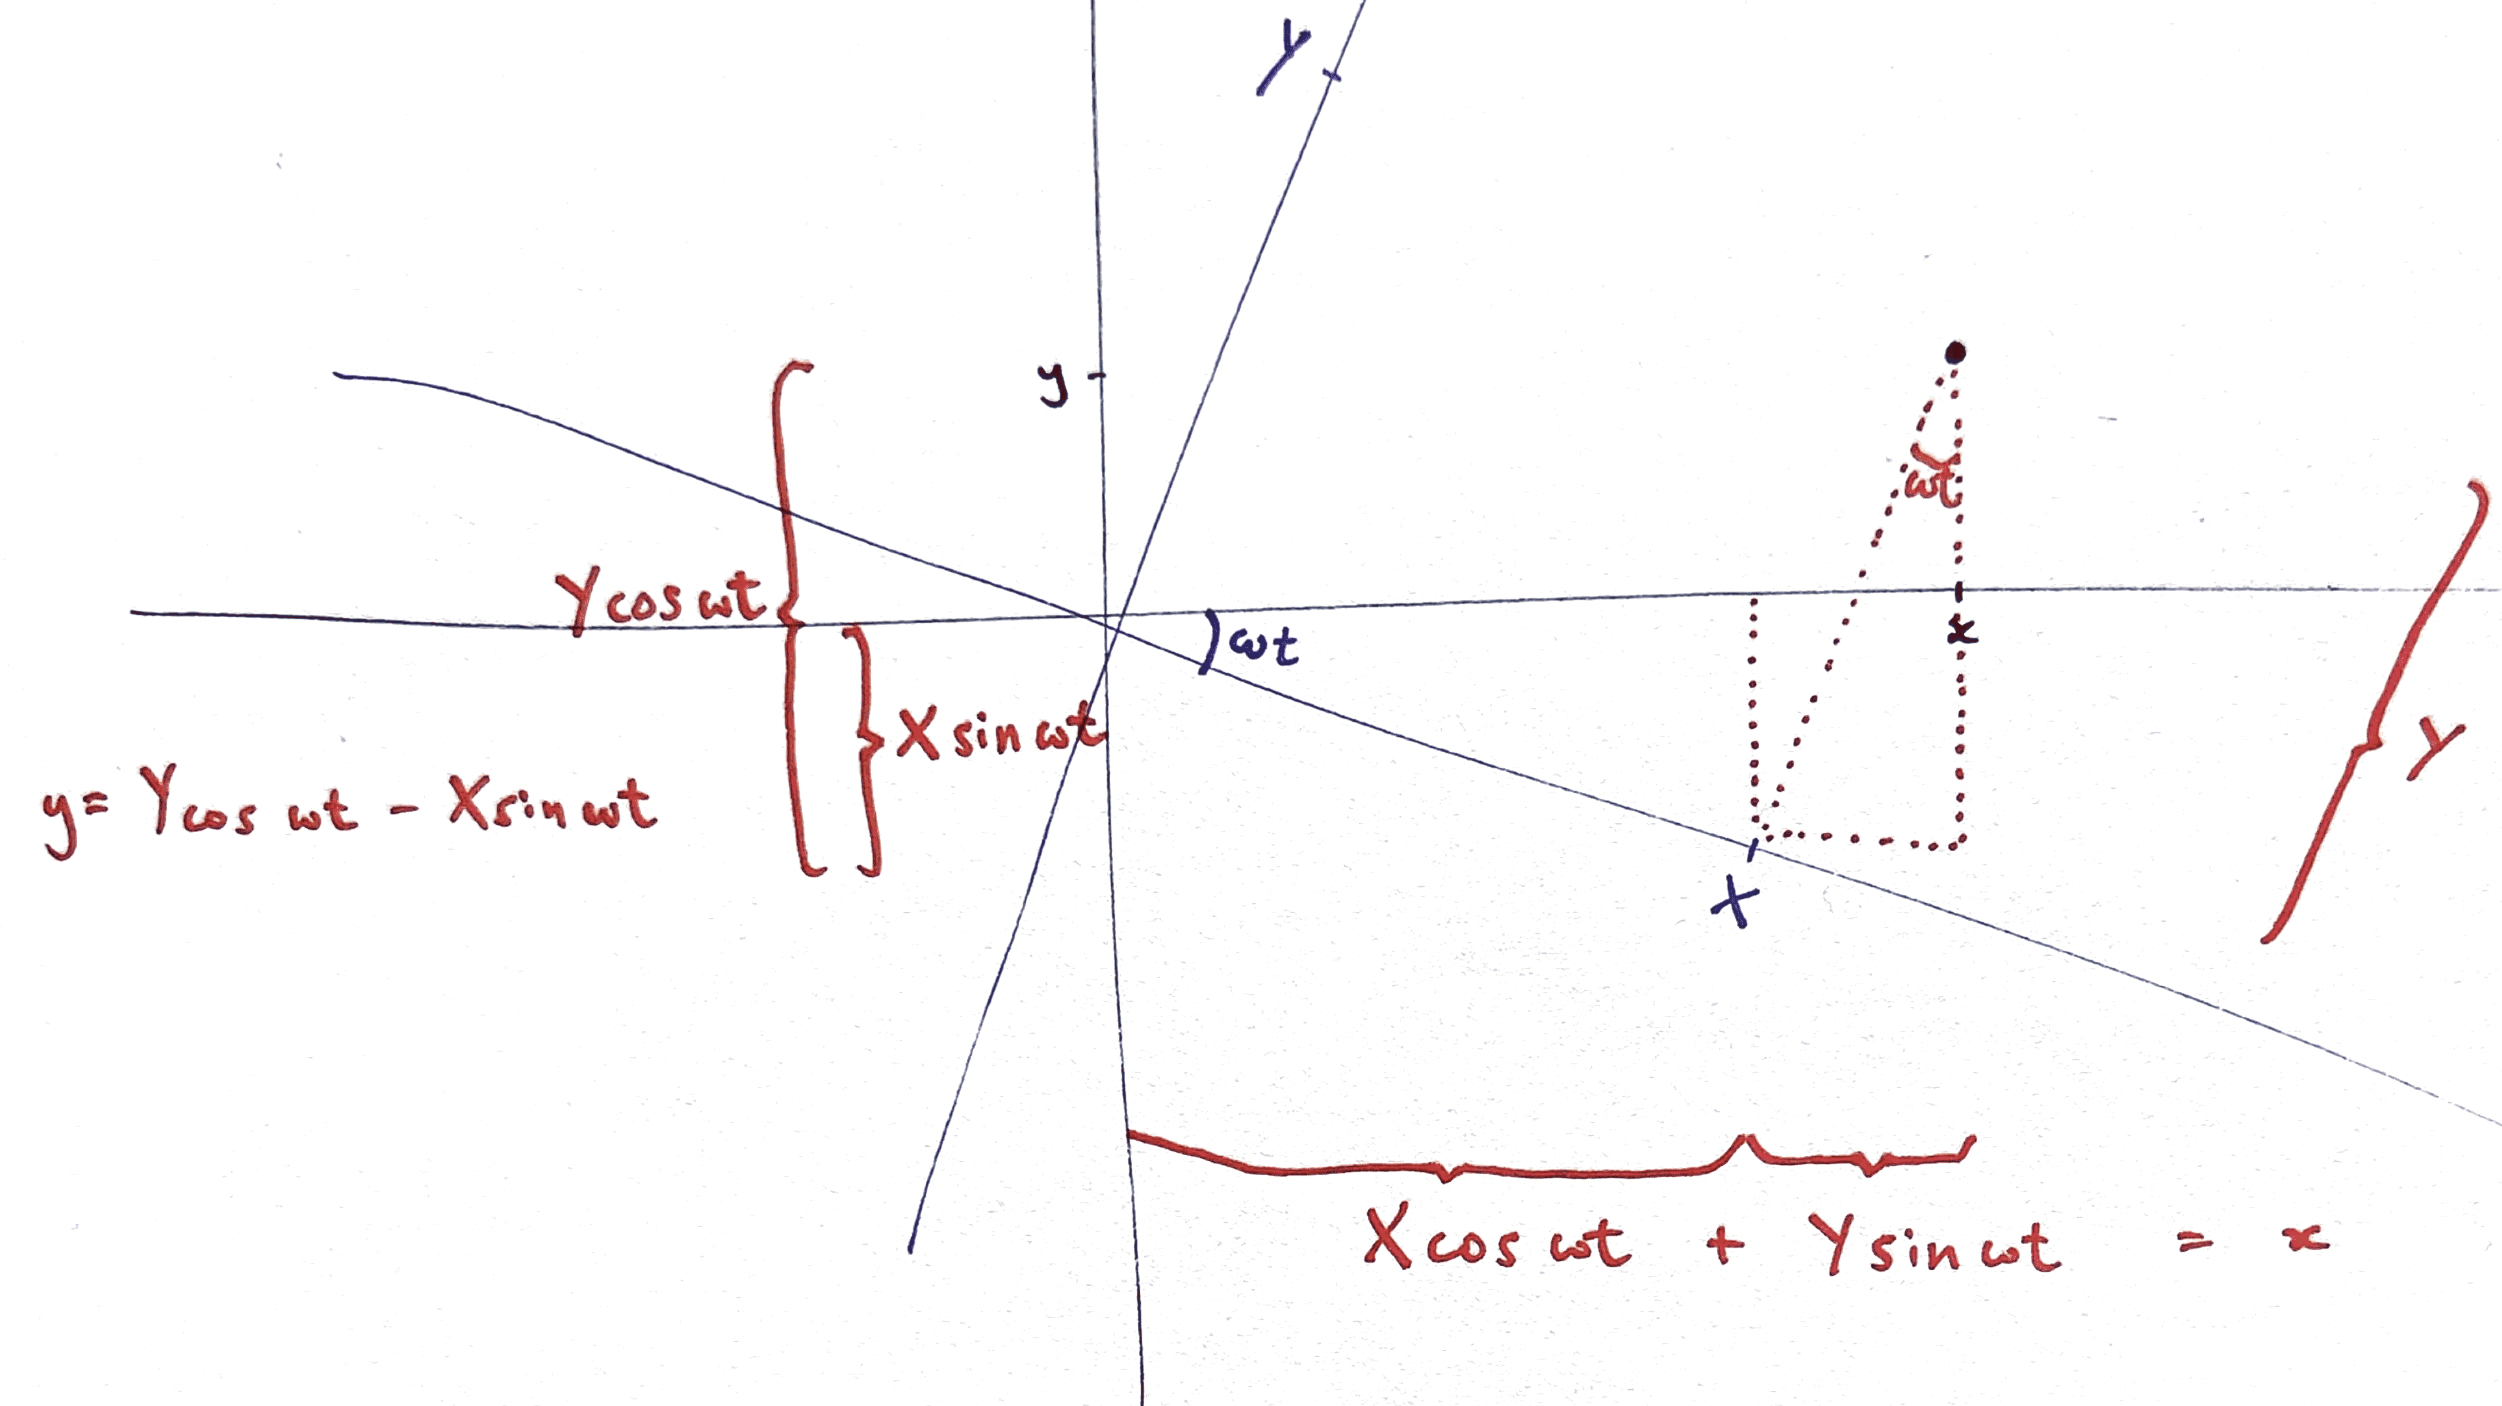
\includegraphics[width=400pt]{img/physics--susskind--the-theoretical-minimum--1.-the-nature-of-classical-mechanics--6.-the-principle-of-least-action--28fe.png}
\end{mdframed}

To translate between the two reference frames:

\begin{align*}
    x &= X \cos \omega t + Y \sin \omega t \\
    y &= -X \sin \omega t + Y \cos \omega t.
  \end{align*}
  i.e.
\begin{align*}
  \vecMM{x}{y} = \matMMxNN{\cos \omega t}{-\sin \omega t}{\sin \omega t}{\cos \omega t} \vecMM{X}{Y}.
\end{align*}

\begin{align*}
  \vecMM{\xdot}{\ydot} =
        \matMMxNN{ \cos \omega t}{-\sin \omega t}{\sin \omega t}{\cos \omega t} \vecMM{\dot{X}}{\dot{Y}} +
  \omega\matMMxNN{-\sin \omega t}{-\cos \omega t}{\cos \omega t}{-\sin \omega t} \vecMM{X}{Y}
\end{align*}
\TODO


Observer A sees a particle moving with no forces acting on it, so the Lagrangian from their point of view
is $\frac{1}{2}m(\xdot^2 + \ydot^2)$.

From observer B's point of view, we have
\begin{align*}
  \xdot &= -\omega X \sin \omega t + \dot{X}\cos \omega t  +  \omega Y \cos \omega t \\
  \ydot &= -\omega X \cos \omega t - \omega Y \sin \omega t,
\end{align*}
therefore
\begin{align*}
    \xdot^2 &= \omega^2\(X^2\sin^2\omega t - 2XY\sin \omega t \cos\omega t + Y^2\cos^2\omega t\) \\
    \ydot^2 &= \omega^2\(X^2\cos^2\omega t + 2XY\sin \omega t \cos\omega t + Y^2\sin^2\omega t\),
\end{align*}
and so the Lagrangian for observer B is
\begin{align*}
  \frac{1}{2}m(\xdot^2 + \ydot^2) =
  \omega^2\frac{1}{2}m(X^2 + Y^2).
\end{align*}

\subsection*{Conjugate momentum}
Note that if $\Lag = \frac{1}{2}\sum_im\xdot_i^2 - V(x_1, \ldots, x_N)$ as usual,
then $\pdLdxdi = m\xdot_i$. Accordingly, $p_i := \pdLdqdi$ is referred to as the ``conjugate momentum''
to $q_i$.

So a streamlined statement of the Euler-Lagrange equations for classical mechanics is
\begin{align*}
  \frac{\d p_i}{\dt} - \pdLdqi = 0.
\end{align*}
\subsection*{Conserved quantities}
Momentum is conserved when there is no potential energy function (which would be dependent on the spatial
coordinates).

In general, if there is a generalized coordinate that appears in the Lagrangian only via its velocity (if there
exists a change of coordinates such that this is true), then the corresponding generalized momentum is
conserved.

\section{7.  Symmetries and Conservation Laws}

\begin{enumerate}
\item $\Lag(\qdot, q) = \frac{1}{2}(\dot{q_1}^2 + \dot{q_2}^2) - V(q_1 - q_2)$
\end{enumerate}
Derive the equations of motion:
\begin{align*}
  \ddt \pdLdqdOne &= \pdLdqOne \\
  \ddt \pdLdqdTwo &= \pdLdqTwo \\
\end{align*}
\begin{align*}
  \dot{p}_1        &= -V'(q_1 - q_2) \\
  \dot{p}_2        &= +V'(q_1 - q_2)
\end{align*}
The sign difference is related to the fact that the potential depends on the distance between the two
particles: they are both approaching each other. This has something to do with Newton's third law.

So $\ddt(p_1 + p_2) = 0$: generalized momentum is conserved.

\item $\Lag(\qdot, q) = \frac{1}{2}(\dot{q_1}^2 + \dot{q_2}^2) - V(aq_1 - bq_2)$
\begin{align*}
  \dot{p}_1        &= -aV'(aq_1 - bq_2) \\
  \dot{p}_2        &= +bV'(aq_1 - bq_2)
\end{align*}
\begin{align*}
  \dot{p}_1 + \dot{p}_2 &= (b-a)V'(aq_1 - bq_2) \\
\end{align*}
Now generalized momentum appears not to be conserved in general.

But we see that $bp_1 + ap_2$ is conserved.
